

\tikzset{every picture/.style={line width=0.75pt}} %set default line width to 0.75pt        

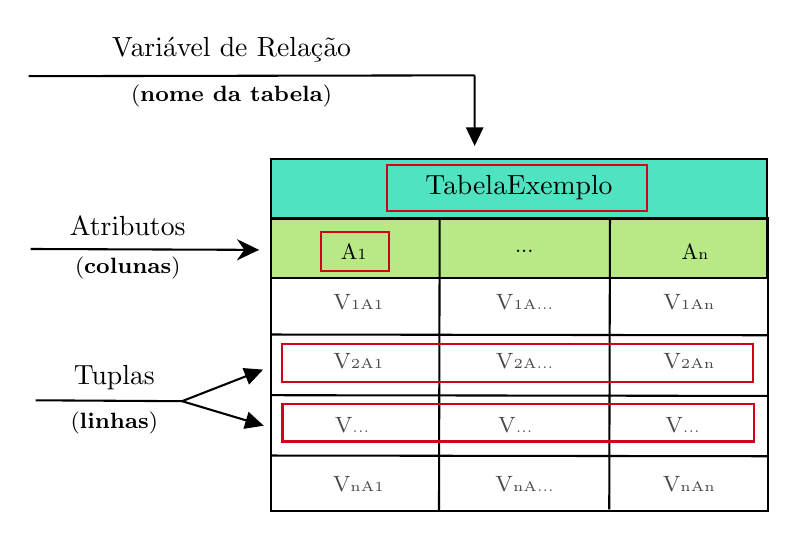
\begin{tikzpicture}[x=0.75pt,y=0.75pt,yscale=-1,xscale=1]
%uncomment if require: \path (0,456.4000015258789); %set diagram left start at 0, and has height of 456.4000015258789

%Shape: Rectangle [id:dp9895438777319416] 
\draw   (199.76,128.06) -- (439.3,128.06) -- (439.3,269.14) -- (199.76,269.14) -- cycle ;
%Straight Lines [id:da9433008870660626] 
\draw    (200.17,183.96) -- (439.3,184.31) ;


%Straight Lines [id:da2966959811071168] 
\draw    (199.96,213.19) -- (439.09,213.54) ;


%Straight Lines [id:da10336227761172356] 
\draw    (199.96,242.26) -- (439.09,242.6) ;


%Shape: Rectangle [id:dp29843450985148356] 
\draw  [fill={rgb, 255:red, 184; green, 233; blue, 134 }  ,fill opacity=1 ] (199.76,128.06) -- (439.07,128.06) -- (439.07,156.8) -- (199.76,156.8) -- cycle ;
%Straight Lines [id:da7072311505307143] 
\draw    (281.21,128) -- (280.87,268.53) ;


%Straight Lines [id:da24303755507006675] 
\draw    (363.25,127.67) -- (362.9,268.19) ;


%Straight Lines [id:da8433947995405431] 
\draw    (84.07,142.75) -- (192.19,143.17) ;
\draw [shift={(194.19,143.18)}, rotate = 180.22] [fill={rgb, 255:red, 0; green, 0; blue, 0 }  ][line width=0.75]  [draw opacity=0] (10.72,-5.15) -- (0,0) -- (10.72,5.15) -- (7.12,0) -- cycle    ;

%Shape: Rectangle [id:dp9829425897866726] 
\draw  [color={rgb, 255:red, 208; green, 2; blue, 27 }  ,draw opacity=1 ] (205.49,217.22) -- (432.44,217.22) -- (432.44,235.51) -- (205.49,235.51) -- cycle ;
%Straight Lines [id:da9003126370670107] 
\draw    (86.49,215.65) -- (157.07,216.08) ;


%Shape: Rectangle [id:dp34368494625131474] 
\draw  [color={rgb, 255:red, 208; green, 2; blue, 27 }  ,draw opacity=1 ] (205.06,188.46) -- (432,188.46) -- (432,206.75) -- (205.06,206.75) -- cycle ;
%Straight Lines [id:da28450929807989755] 
\draw    (157.07,216.08) -- (194.24,201.59) ;
\draw [shift={(196.1,200.87)}, rotate = 518.71] [fill={rgb, 255:red, 0; green, 0; blue, 0 }  ][line width=0.75]  [draw opacity=0] (8.93,-4.29) -- (0,0) -- (8.93,4.29) -- cycle    ;

%Straight Lines [id:da38844388554414944] 
\draw    (157.07,216.08) -- (194.52,227.29) ;
\draw [shift={(196.43,227.87)}, rotate = 196.67000000000002] [fill={rgb, 255:red, 0; green, 0; blue, 0 }  ][line width=0.75]  [draw opacity=0] (8.93,-4.29) -- (0,0) -- (8.93,4.29) -- cycle    ;

%Straight Lines [id:da6694551113867799] 
\draw    (83.2,59.49) -- (298.05,59.09) ;


%Shape: Rectangle [id:dp5574880153243091] 
\draw  [fill={rgb, 255:red, 80; green, 227; blue, 194 }  ,fill opacity=1 ] (199.76,99.32) -- (439.07,99.32) -- (439.07,128.06) -- (199.76,128.06) -- cycle ;
%Straight Lines [id:da8765291155015824] 
\draw    (298.05,59.09) -- (298.06,91.08) ;
\draw [shift={(298.06,93.08)}, rotate = 269.98] [fill={rgb, 255:red, 0; green, 0; blue, 0 }  ][line width=0.75]  [draw opacity=0] (8.93,-4.29) -- (0,0) -- (8.93,4.29) -- cycle    ;

%Shape: Rectangle [id:dp31459180611157866] 
\draw  [color={rgb, 255:red, 208; green, 2; blue, 27 }  ,draw opacity=1 ] (255.94,102.46) -- (381.06,102.46) -- (381.06,124.63) -- (255.94,124.63) -- cycle ;
%Shape: Rectangle [id:dp48382611043878065] 
\draw  [color={rgb, 255:red, 208; green, 2; blue, 27 }  ,draw opacity=1 ] (224.14,134.4) -- (256.9,134.4) -- (256.9,153.28) -- (224.14,153.28) -- cycle ;

% Text Node
\draw (239.74,144.01) node [scale=0.8] [align=left] {A{\scriptsize 1}};
% Text Node
\draw (321.96,144.01) node [scale=0.8] [align=left] {...};
% Text Node
\draw (404.18,144.01) node [scale=0.8] [align=left] {A{\scriptsize n}};
% Text Node
\draw (241.98,168.48) node [scale=1,color={rgb, 255:red, 74; green, 74; blue, 74 }  ,opacity=1 ] [align=left] {{\footnotesize V}{\tiny 1A1}};
% Text Node
\draw (130.91,131.43) node [scale=1] [align=left] {Atributos};
% Text Node
\draw (130.91,151.67) node [scale=1] [align=left] {{\footnotesize (\textbf{colunas})}};
% Text Node
\draw (241.98,196.46) node [scale=1,color={rgb, 255:red, 74; green, 74; blue, 74 }  ,opacity=1 ] [align=left] {{\footnotesize V}{\tiny 2A1}};
% Text Node
\draw (238.98,227.67) node [scale=1,color={rgb, 255:red, 74; green, 74; blue, 74 }  ,opacity=1 ] [align=left] {{\footnotesize V}{\tiny ...}};
% Text Node
\draw (241.98,256.17) node [scale=1,color={rgb, 255:red, 74; green, 74; blue, 74 }  ,opacity=1 ] [align=left] {{\footnotesize V}{\tiny nA1}};
% Text Node
\draw (322.14,168.48) node [scale=1,color={rgb, 255:red, 74; green, 74; blue, 74 }  ,opacity=1 ] [align=left] {{\footnotesize V}{\tiny 1A...}};
% Text Node
\draw (322.14,196.46) node [scale=1,color={rgb, 255:red, 74; green, 74; blue, 74 }  ,opacity=1 ] [align=left] {{\footnotesize V}{\tiny 2A...}};
% Text Node
\draw (317.64,227.67) node [scale=1,color={rgb, 255:red, 74; green, 74; blue, 74 }  ,opacity=1 ] [align=left] {{\footnotesize V}{\tiny ...}};
% Text Node
\draw (322.14,256.17) node [scale=1,color={rgb, 255:red, 74; green, 74; blue, 74 }  ,opacity=1 ] [align=left] {{\footnotesize V}{\tiny nA...}};
% Text Node
\draw (401.22,168.48) node [scale=1,color={rgb, 255:red, 74; green, 74; blue, 74 }  ,opacity=1 ] [align=left] {{\footnotesize V}{\tiny 1An}};
% Text Node
\draw (401.22,196.46) node [scale=1,color={rgb, 255:red, 74; green, 74; blue, 74 }  ,opacity=1 ] [align=left] {{\footnotesize V}{\tiny 2An}};
% Text Node
\draw (398.22,227.67) node [scale=1,color={rgb, 255:red, 74; green, 74; blue, 74 }  ,opacity=1 ] [align=left] {{\footnotesize V}{\tiny ...}};
% Text Node
\draw (401.22,256.17) node [scale=1,color={rgb, 255:red, 74; green, 74; blue, 74 }  ,opacity=1 ] [align=left] {{\footnotesize V}{\tiny nAn}};
% Text Node
\draw (124.43,204.59) node [scale=1] [align=left] {Tuplas};
% Text Node
\draw (124.43,226.56) node [scale=1] [align=left] {{\footnotesize (\textbf{linhas})}};
% Text Node
\draw (180.93,46.33) node [scale=1] [align=left] {Variável de Relação};
% Text Node
\draw (180.93,69.05) node [scale=1] [align=left] {{\footnotesize (\textbf{nome da tabela})}};
% Text Node
\draw (319.41,113.34) node [scale=1] [align=left] {TabelaExemplo};


\end{tikzpicture}
